%\chapter{Supercondensadores}
El almacenar energía eléctrica es uno de los mayores problemas a la hora de diseñar sistemas electrónicos tanto móviles como estacionarios, los requerimientos varían de acuerdo a las necesidades de cada uno, en general es un \textit{trade-off} entre densidad de energía (cuánta energía se puede almacenar) y densidad de potencia (que tan rápido puede ser entregada la energía almacenada). Para poner en perspectiva las tecnologías de almacenamiento de energía, existe el diagrama de Ragone (ver figura \ref{fig:ragone}).Las celdas de combustible (\textit{Fuel Cells}), entregan la mayor densidad de energía, pero son complicadas, mientras que las baterías poseen mayor densidad de potencia, pierden capacidad con los ciclos de carga y descarga. Los supercondensadores van un paso más allá, aumentado la densidad de potencia y aportando mayor vida útil, entregando una nueva posibilidad a la hora de diseñar sistemas eléctricos, ya como fuente de energía por sí mismo, o en sistemas híbridos combinados con otras tecnologías \citep{Thounthong2009}.\\
Un supercondensador es un condensador que exhibe una capacitancia mucho mayor a la de un condensador normal (fácilmente 1000 veces mayor). No utilizan un material dieléctrico, si no, una doble capa electrostática y la llamada pseudocapacitancia electroquímica. Estos dispositivos están compuestos por dos electrodos de un material de gran área superficial específica, separados por una membrana permeable empapada en electrolíto (ver figura \ref{fig:edlc}). Si la capacidad del dispositivo surge de la separación de cargas en una doble capa electrostática de Helmholtz, se habla de condensadores de doble capa. Por otro lado, si la capacitancia surge de reacciones farádicas en los electródos, se denominan pseudocondensadores, más aún, si la capacitancia surge de una doble capa y de reacciones farádicas, se tienen supercondensadores híbridos.

\begin{figure}
	\centering
	\fbox{
		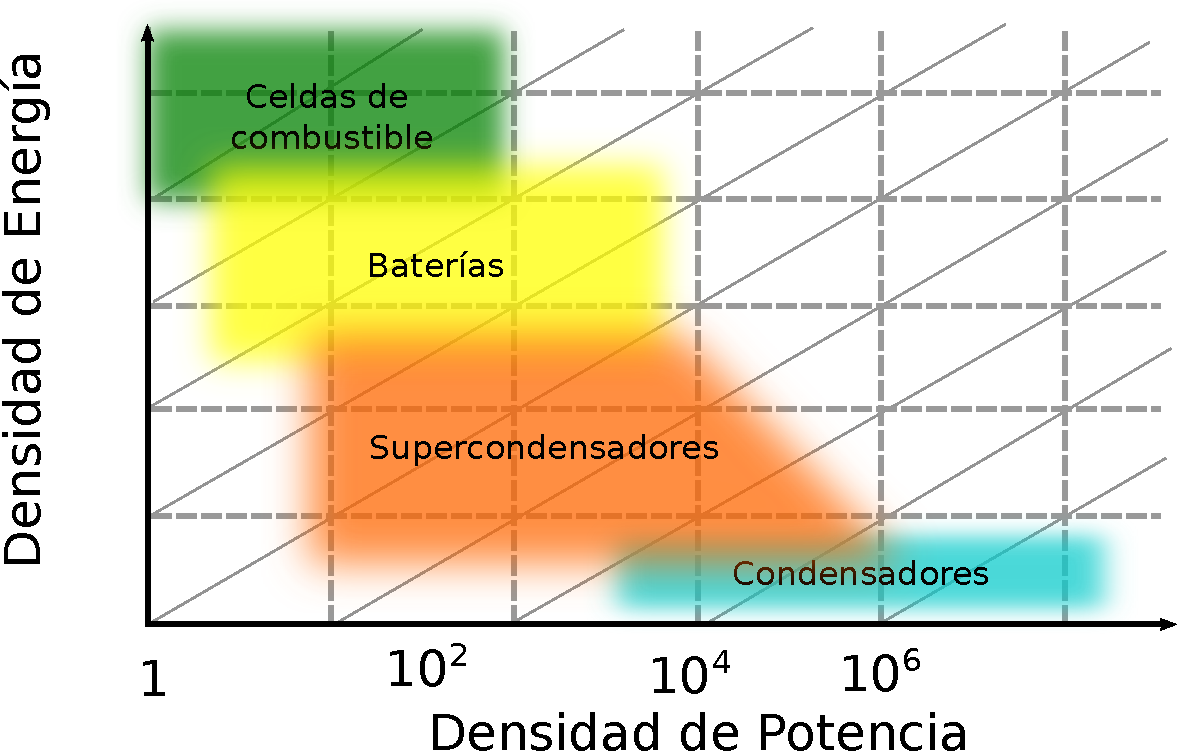
\includegraphics[width = 0.7\textwidth]{ragone.pdf}
	}
	\caption[Diagrama de Ragone]{El diagrama de Ragone compara diferentes tecnologías de almacenamiento de energía de acuerdo a su densidad de potencia y densidad de energía.}
	\label{fig:ragone}
\end{figure}

\section{El condensador ideal}
Generalmente un condensador se modela como un par de placas paralelas separadas por un dieléctrico, éste es definido por su capacitancia, la que refleja a groso modo, su capacidad de almacenar energía. Del modelo de placas paralelas se desprende la definición de capacitancia $C$ como la razón entre la magnitud de carga en cada placa $Q$ y el voltaje entre los terminales $V$:

\begin{equation}
	C = \frac{Q}{V}
\end{equation}

Esta magnitud, no depende del voltaje o corriente del condensador, si no, de su construcción. Para fines prácticos, el condensador ideal como componente electrónico es modelado por la ecuación que relaciona la corriente\footnote{En estricto rigor, no hay corriente en el condensador, pues los electrones no ``saltan'' de una placa a otra, sólo se acumulan en una de ellas. La corriente en el condensador, es más bien una corriente de desplazamiento.} con el voltaje en los terminales del dispositivo, considerando que $i = dq/dt$:

\begin{equation}
	i(t) = C \frac{dv(t)}{dt}
\end{equation}

Para corrientes constantes, el voltaje varía linealmente como en el gráfico de carga y descarga de la figura \ref{fig:plot:charge-discharge_ideal_cap}.

\begin{figure}
	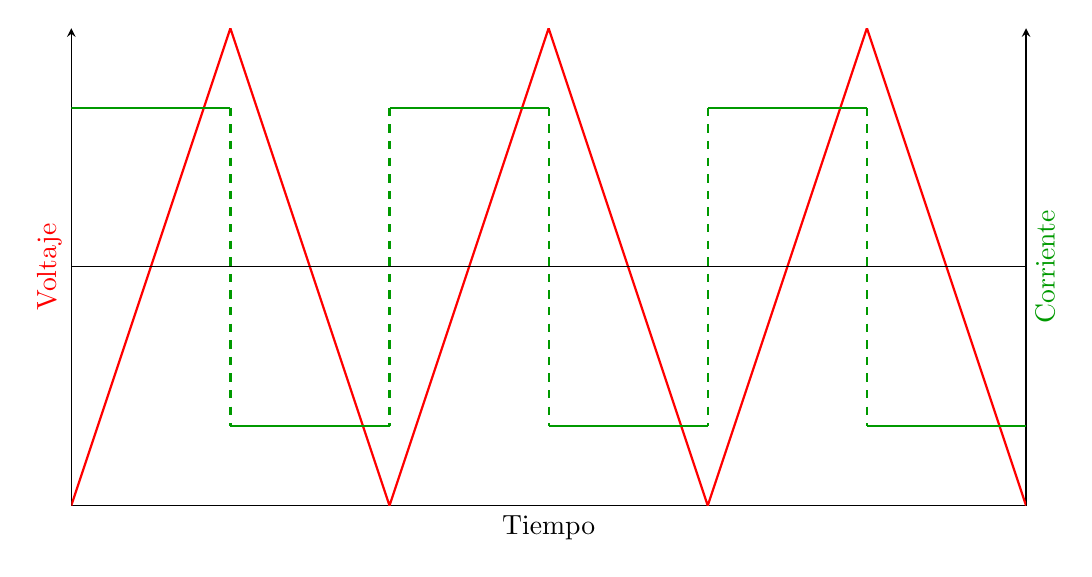
\begin{tikzpicture}
	% let both axes use the same layers
	\pgfplotsset{set layers, 	width=\textwidth, height = 0.5\textwidth}
	
	\begin{axis}[
	scale only axis,
	axis y line=left, % the ’*’ avoids arrow heads
	axis x line*=bottom,
	xlabel=Tiempo,
	ylabel={\color{red} Voltaje},
	no markers,
	xmin=0,
	xmax=6,
	cycle list name=exotic,
	ticks=none,
	]
		\addplot [red, thick] table {
			A B
			%charge
			0 -1
			1  1
			
			2 -1
			3  1
			
			4 -1
			5  1
			
			%discharge
			1  1			
			2 -1
			
			3  1
			4 -1
			
			5  1
			6 -1
		};	
	\end{axis}
	\begin{axis}[
	scale only axis,
	axis y line=right,
	axis x line=none,
	ylabel={\color{green!60!black} Corriente},
	ymin = -1.5,
	ymax = 1.5,
	xmin = 0,
	xmax = 6,
	no markers,
	ticks=none,
	]
		\addplot [green!60!black, thick] table {
			A B
			0  1
			1  1
			
			1 -1
			2 -1
			
			2  1
			3  1
			
			3 -1
			4 -1
			
			4  1
			5  1
			
			5 -1
			6 -1	
		};
		\addplot [green!60!black, thick, dashed] table {
			A B
			1  1
			1 -1

			2  1
			2 -1
			
			3  1
			3 -1
			
			4  1
			4 -1
			
			5  1
			5 -1
		};
		\addplot [black] table {
			0  0
			6  0
		};
	\end{axis}
	\end{tikzpicture}
	\caption{Carga y descarga de un condensador ideal a corriente constante.}
	\label{fig:plot:charge-discharge_ideal_cap}
\end{figure}

\section{El condensador real}
Un condensador ideal almacenaría energía al cargarse y la entregaría al descargarse sin ninguna disipación, es decir, su eficiencia sería del 100\%, podría soportar cualquier voltaje aplicado o cargarse y descargarse por una corriente cuan grande se desee.  En realidad, los condensadores sí disipan energía, poseen voltajes de operación y corrientes máximas de carga y descarga. Todo esto depende de como fue construido y qué materiales se utilizaron.\\
El voltaje máximo de operación de un condensador convencional dieléctrico, es determinado por la tensión de ruptura del material\footnote{Voltaje al cual se pierden las propiedades dieléctricas del material, provocando cortocircuito al interior del dispositivo. Este está determinado por la fuerza dieléctrica y el espesor del material. En condensadores electrolíticos, la tensión de ruptura está determinada por otros mecanismos \citep{Yahalom1971}.}. En lo que respecta a los supercondensadores, el voltaje máximo de carga depende fundamentalmente de electrolíto usado, principalmente por las reacciones que ocurren a ciertos potenciales.\\

\subsection{Resistencia en serie equivalente (ESR)}
Las imperfecciones en la construcción de los electrodos, y la naturaleza de los materiales utilizados (e.g. resistencia no cero), disipan energía durante la carga y descarga como si se tratase de una resistencia en serie al condensador, esto se ve reflejado como una caída de voltaje en los terminales del dispositivo (figura \ref{fig:plot:charge-discharge_esr}), y disminuye la eficiencia de éste.

\begin{figure}
	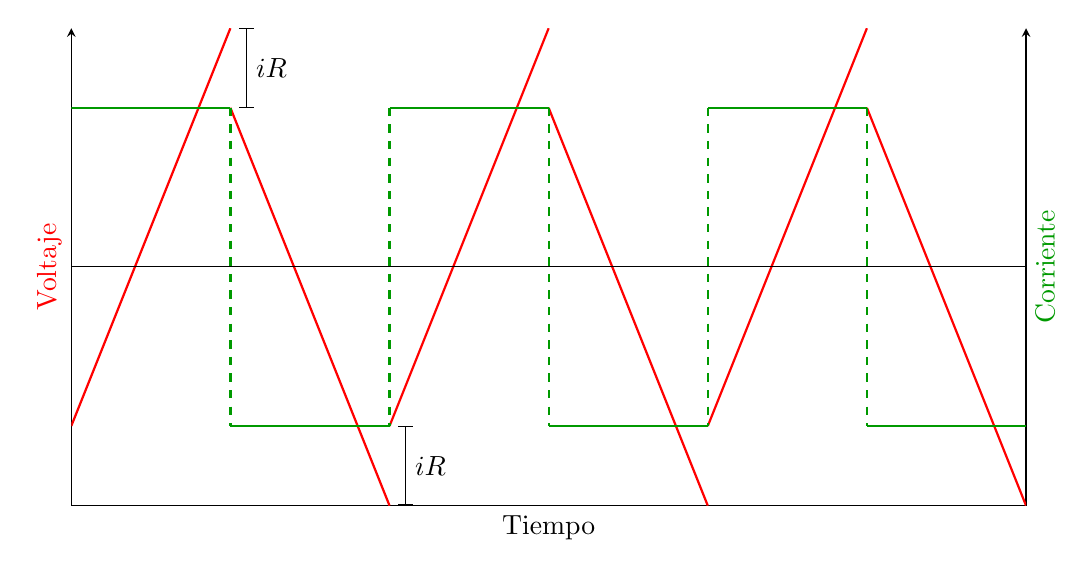
\begin{tikzpicture}
	% let both axes use the same layers
	\pgfplotsset{set layers, 	width=\textwidth, height = 0.5\textwidth}
	
	\begin{axis}[
	scale only axis,
	axis y line=left, % the ’*’ avoids arrow heads
	axis x line*=bottom,
	xlabel=Tiempo,
	ylabel={\color{red} Voltaje},
	no markers,
	xmin=0,
	xmax=6,
	cycle list name=exotic,
	ticks=none,
	]
	\addplot [red, thick] table {
		A B
		%charge
		0 -0.8
		1  1.2
		
		2 -0.8
		3  1.2
		
		4 -0.8
		5  1.2
		
		%discharge
		1  0.8			
		2 -1.2
		
		3  0.8
		4 -1.2
		
		5  0.8
		6 -1.2
	};	
	\draw [arrows={|-|}] (axis cs:1.1,1.2) -- node[right]{$iR$} (axis cs:1.1,0.8);
	\draw [arrows={|-|}] (axis cs:2.1,-1.2) -- node[right]{$iR$} (axis cs:2.1,-0.8);
	\end{axis}
	\begin{axis}[
	scale only axis,
	axis y line=right,
	axis x line=none,
	ylabel={\color{green!60!black} Corriente},
	ymin = -1.5,
	ymax = 1.5,
	xmin = 0,
	xmax = 6,
	no markers,
	ticks=none,
	]
	\addplot [green!60!black, thick] table {
		A B
		0  1
		1  1
		
		1 -1
		2 -1
		
		2  1
		3  1
		
		3 -1
		4 -1
		
		4  1
		5  1
		
		5 -1
		6 -1	
	};
	\addplot [green!60!black, thick, dashed] table {
		A B
		1  1
		1 -1
		
		2  1
		2 -1
		
		3  1
		3 -1
		
		4  1
		4 -1
		
		5  1
		5 -1
	};
	\addplot [black] table {
		0  0
		6  0
	};
	\end{axis}
	\end{tikzpicture}
	\caption{Carga y descarga de un condensador evidenciando el efecto de una ESR.}
	\label{fig:plot:charge-discharge_esr}
\end{figure}



\subsection{Corriente de fuga (\emph{leakage current})}
Entre los electrodos del condensador fluye una corriente no deseada cuando existe una diferencia de potencial entre los electrodos (cuando el condensador está cargado), esta corriente descarga al condensador incluso si está desconectado. Esta imperfección es modelada como una resistencia en paralelo al condensador.

\subsection{Circuito equivalente}
El comportamiento de los condensadores reales (convencionales o electroquímicos), son modeladas por un circuito equivalente, donde se introducen componentes que representan las imperfecciones del funcionamiento del condensador real.\\
El modelo de circuito equivalente más sencillo para un supercondensador, es incluir una resistencia en paralelo al condensador, que represente la corriente de fuga, y una resistencia en serie.

\begin{figure}
	\centering
	\fbox{
		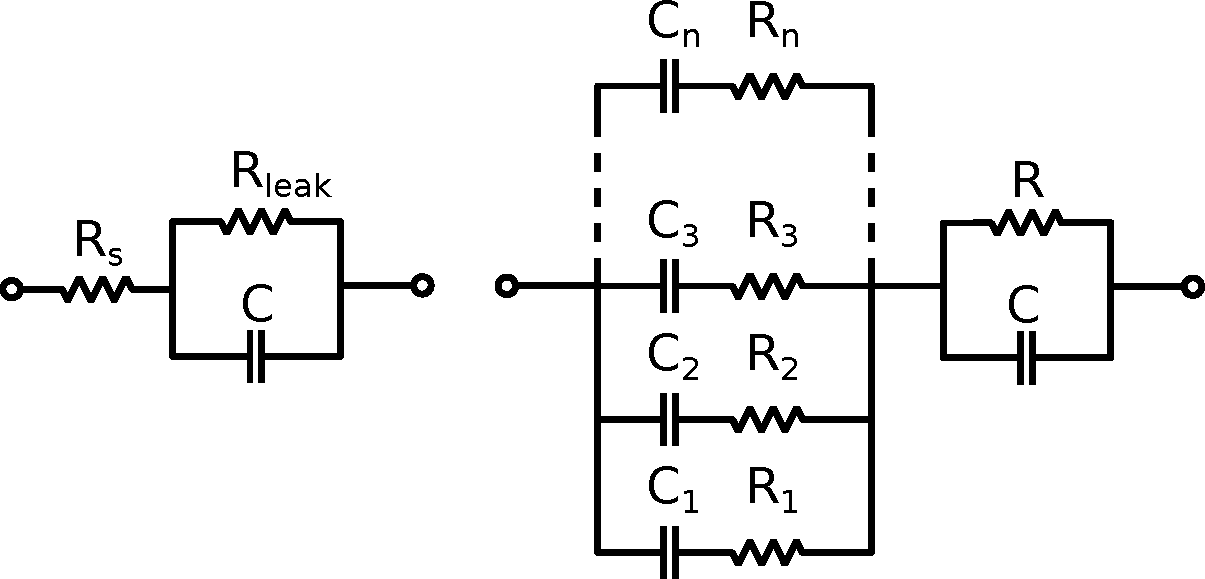
\includegraphics[width=0.7\textwidth]{equivalent_both.pdf}
		}
	\caption{Izquierda: Circuito equivalente sencillo. Derecha: Circuito equivalente complejizado \citep{Fletcher2014}.}
	\label{fig:equiv_both}
\end{figure}

\section{¿Qué hace a un supercondensador súper?}
La densidad de energía de un supercondensador comparada a la de un condensador convencional es varios órdenes de magnitud superior, a modo de comparación, generalmente se utilizan microfaradios (10$^{-6}$ Faradios), para medir la capacidad de un condensador convencional, mientras que en un supercondensador es común ver capacidades de cientos de Faradios. Esta característica le otorga el grado de súper a los supercondensadores.

\subsection{Doble capa electrostática de Helmholtz\index{doble capa de Helmholtz}}
La gran densidad de energía de un supercondensador tiene que surgir de algún mecanismo de almacenamiento de cargas. A diferencia de las baterías, este mecanismo es puramente físico, pues no hay reacciones químicas en los electrodos, las cargas son separadas en lo que Helmholtz llamó \emph{Doble capa electrónica} \citep{Frackowiak2001}, así, los supercondensadores también son llamados EDLCs (del inglés \emph{Electric Double Layer Capacitor}).

\begin{figure}[h!]
	\centering
	\fbox{
		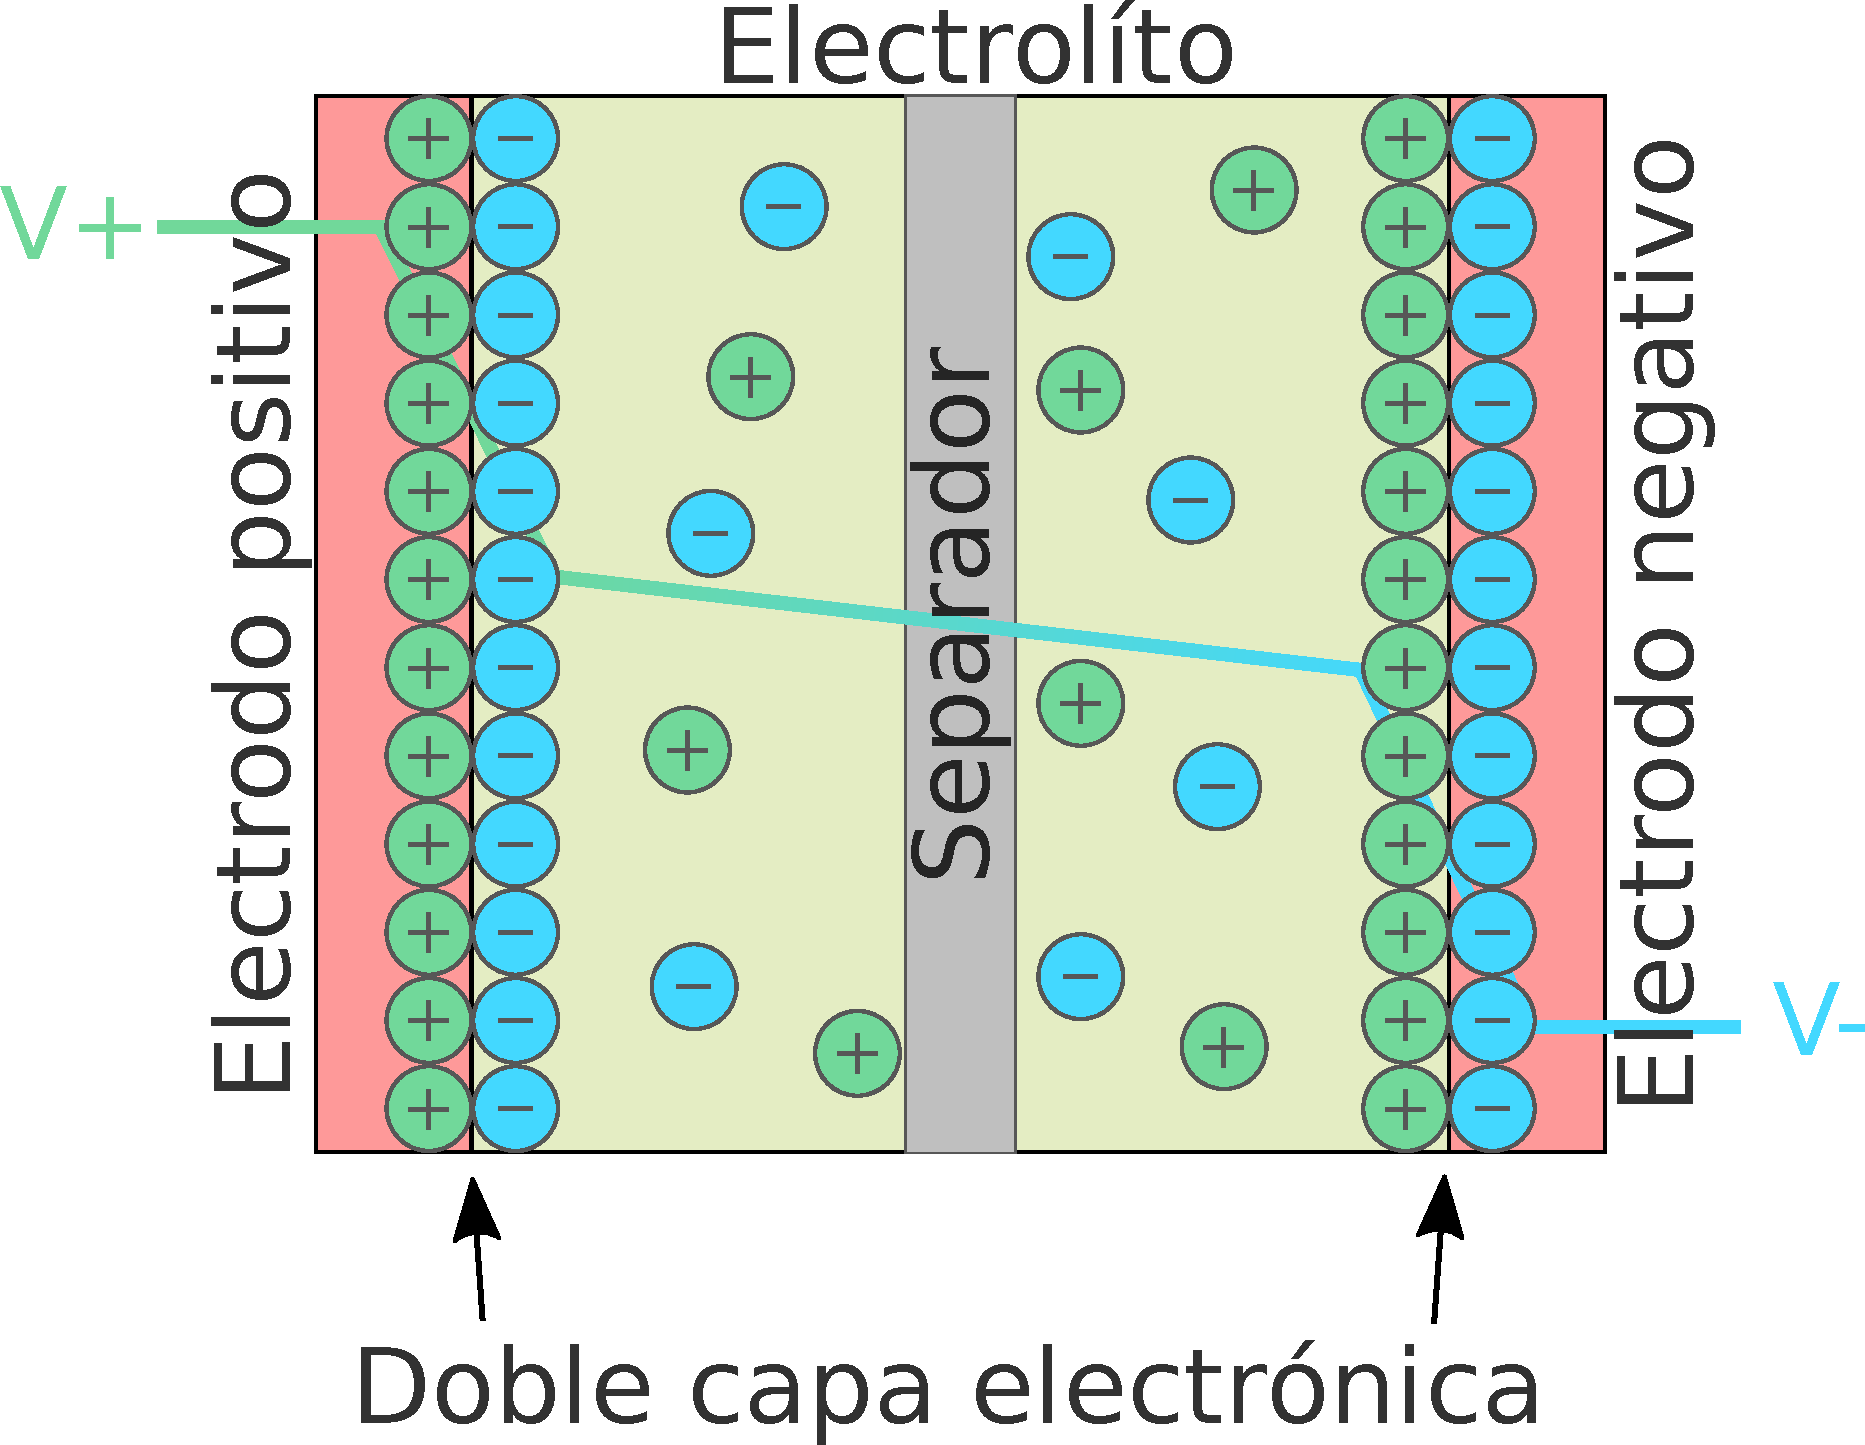
\includegraphics[width=0.7\textwidth]{edlc_schem.pdf}
		}
	\caption{Esquema de un supercondensador mostrando una doble capa electrónica de Helmholtz en cada electrodo y el perfil del potencial eléctrico en él.}
	\label{fig:edlc}
\end{figure}

\subsection{Pseudocapacitancia}
Cuando en un supercondensador existe intercambio de electrones entre los electrodos y el electrolítico (reacciones farádicas), se habla de pseudocapacitancia. El intercambio de electrones 


\section{Mediciones en supercondensadores}

\subsection{Voltametría cíclica}
En una voltametría cíclica convencional, se varía el potencia entre los electrodos de manera lineal y se mide la corriente, típicamente el barrido de voltaje se realiza entre dos voltajes fijos, y el recorrido se hace de ida y vuelta. Los parámetros importantes en la voltametría cíclica son: voltajes límite inferior y superior, velocidad de barrido.

La capacitancia específica puede ser calculada de la voltametría cíclica según la ecuación \ref{eq:cyclic_voltametry}\footnote{Esta ecuación corresponde a la carga total ($\int i dv / \nu$), dividida por la ventana de potencial $\Delta V$, el factor $2$ surge de que la voltametría cíclica comprende tanto un ciclo de carga como uno de descarga.}.

\begin{equation}\label{eq:cyclic_voltametry}
	C_{s} = \frac{\int_{V_i}^{V_f}i(v) \; dv}{2 \; \Delta V \; m \; \nu }
\end{equation}

\subsection{Espectroscopía de impedancia electroquímica}
Una señal sinusoidal (corriente o voltaje), de determinada amplitud y frecuencia, se aplica en los terminales del dispositivo midiendo la respuesta (voltaje o corriente según corresponda, junto con el desfase), así, se obtiene la impedancia del sistema a determinada frecuencia. Haciendo un barrido en frecuencia que puede ir desde los milihertz hasta los megahertz, se obtiene el espectro de impedancia del dispositivo. Una forma de representación de los datos obtenidos es el gráfico de Nyquist, un gráfico paramétrico con la frecuencia como parámetro de barrido, donde el eje de las abscisas representa la parte real de la impedancia y las coordenadas la parte imaginaria. Cualitativamente la forma de la curva obtenida puede servir para asignarle un circuito equivalente al dispositivo estudiado, sin embargo, también es posible calcular algunas cantidades, como la resistencia en serie equivalente.

\subsection{Carga y descarga cíclica}
Aquí se aplica una corriente constante para cargar el condensador hasta un potencial preestablecido, cuando se alcanza dicho potencial, se comienza la descarga aplicando una corriente igual a la de carga pero en sentido contrario hasta alcanzar un potencial inferior predefinido. De las curvas obtenidas se puede determinar la capacitancia del condensador, y la resistencia en serie equivalente (ESR). Al extender la medición a miles de ciclos (hasta 10.000 ciclos), se puede determinar cómo será el comportamiento del dispositivo al pasar el tiempo.
De esta medición se puede calcular la capacitancia y la resistencia en serie equivalente.